\documentclass{article}
\usepackage[utf8]{inputenc}
\usepackage{caption}
\usepackage{graphicx}
\usepackage{listings}
\usepackage{amsmath}
\usepackage[framed,numbered,autolinebreaks,useliterate]{mcode}

\title{ENGN4528 Computer Vision Clab3 Report}
\author{Zhipeng Bao ~~ u6600985}
\date{April 2018}

\begin{document}

\maketitle

\section*{Task 1: Face Recognition using eigenface technique}

\subsubsection*{Step 1: Have a look at the training and test pictures}
For this step, I just ran the given $viewyalefaces()$ function. The following 3 figures show the results of the training images and test images. Figure 1 shows a single training image, Figure 2 shows 2 sets of training images of the same person and Figure 3 shows the 10 test images.

\begin{figure}[htbp]
    \centering
    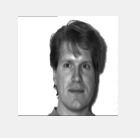
\includegraphics[scale = 0.5]{t10.png}
    \caption{A single image of the training set}
    \label{fig1}
\end{figure}

\begin{figure}[htbp]
    \centering
    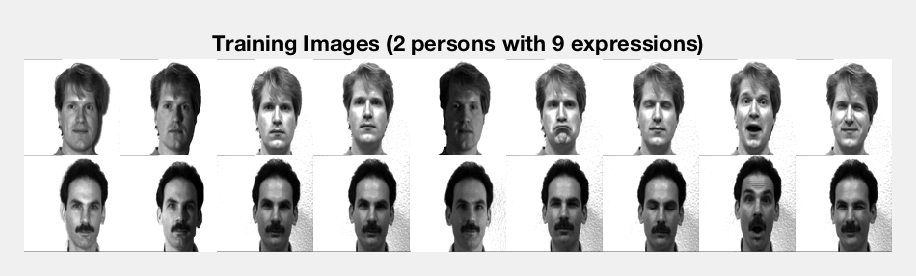
\includegraphics[scale = 0.4]{t11.png}
    \caption{Two sets of images of the training corpus}
    \label{fig2}
\end{figure}

\begin{figure}[htbp]
    \centering
    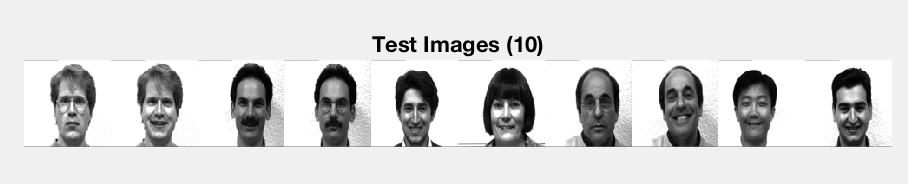
\includegraphics[scale = 0.4]{t12.png}
    \caption{Test images}
    \label{fig3}
\end{figure}

\subsubsection*{Step 2: Train eigenfaces}
For this step, I first re-aligned and restored the training images. Figure 4 shows one of the re-aligned images. Then I read in all the images and for each single image, I treat it as a fixed length 1-D vector. Thus, after reading all the images we can get a training matrix
$$M\in R^{l\times c}$$ 
in which $l$ is the length of the vector and c is the amount of the training images. 

\begin{figure}[htbp]
    \centering
    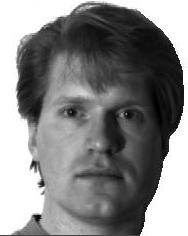
\includegraphics[scale = 0.4]{train_02.jpg}
    \caption{One re-aligned and resized training image}
    \label{fig4}
\end{figure}

The following codes show the process of getting training matrix. Besides, to make the result more accurate, I remove the DC components of the training matrix.

\begin{lstlisting}
%step1: have a look at the training images
dir_name = './trainingset/';
dir_lst = dir(dir_name);
l = length(dir_lst);

top = 10;

%step2: train eigenfaces
train_matrix = [];
count = 0;
%get the train matrix
for i = 1:l
   name = dir_lst(i).name;
   if name(1)=='s'
       img = imread([dir_name,name]);
       [a,b] = size(img);
       img = reshape(img,[a*b 1]);
       img = double(img);
       train_matrix = [train_matrix,img];
       count = count+1;
   end
end

%remove DC Component
mean_face = mean(train_matrix,2);
train_matrix = train_matrix - repmat(mean_face,1,count);

\end{lstlisting}

Then goes to the most important parts of the this task: find the principal components of the training faces.

After loading images, we get a training matrix $M\in R^{45045\times 135}$. To get the principal components of it, we need to calculate the eigen value and eigen vector of $M*M'$. It is quite a complicated task for Matlab. As we just need several ``Principal Component", we can play a trick on it. That is we can calculate the eigen values and eigen vectors of $M'*M$ instead. Next, I will prove $M'*M$ and $M*M'$ have the same eigen values and their eigen vectors have some relations.

Let's assume $V$ is the eigen vector of $MM'$ and thus:
$$MM'V = aV$$
Left multiply $M'$ in both sides, then we can get:
$$M'MM'V = M'aV = aM'V $$
$$M'M(M'V) = a(M'V)$$

So that $a$ is also the eigen value of $M'M$ and the corresponding eigen vector is $M'V$. 

Based on this, I conduct the following $[eig_face] = eigenfaces(C,k)$ function to get the eigenfaces.

\begin{lstlisting}
function [eig_face] = eigenfaces(C,k)
%% returns top K eigenfaces

% calculate eigenvalues
[V,D] = eig(C);
%arrange the eigen values in descend order.
[eig_val,ind] = sort(diag(D),'descend');
eig_vec = V(:,ind);
% take top k vectors
if size(eig_vec,2) >= k
    eig_face = eig_vec(:,1:k);
else
    error('Not enough eigenvectors - check image matrix');
end
\end{lstlisting}

Figure 5 and Figure 6 show the top 5 and top 10 eigenfaces.

\begin{figure}[htbp]
    \centering
    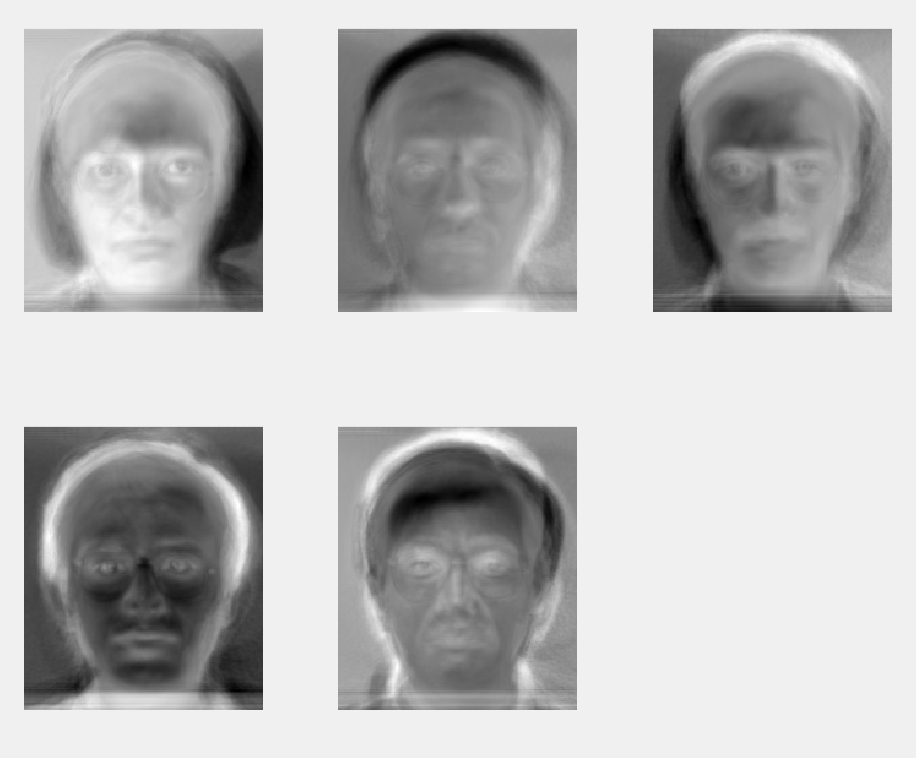
\includegraphics[scale = 0.4]{5.png}
    \caption{Top 5 eigenfaces}
    \label{fig5}
\end{figure}

\begin{figure}[htbp]
    \centering
    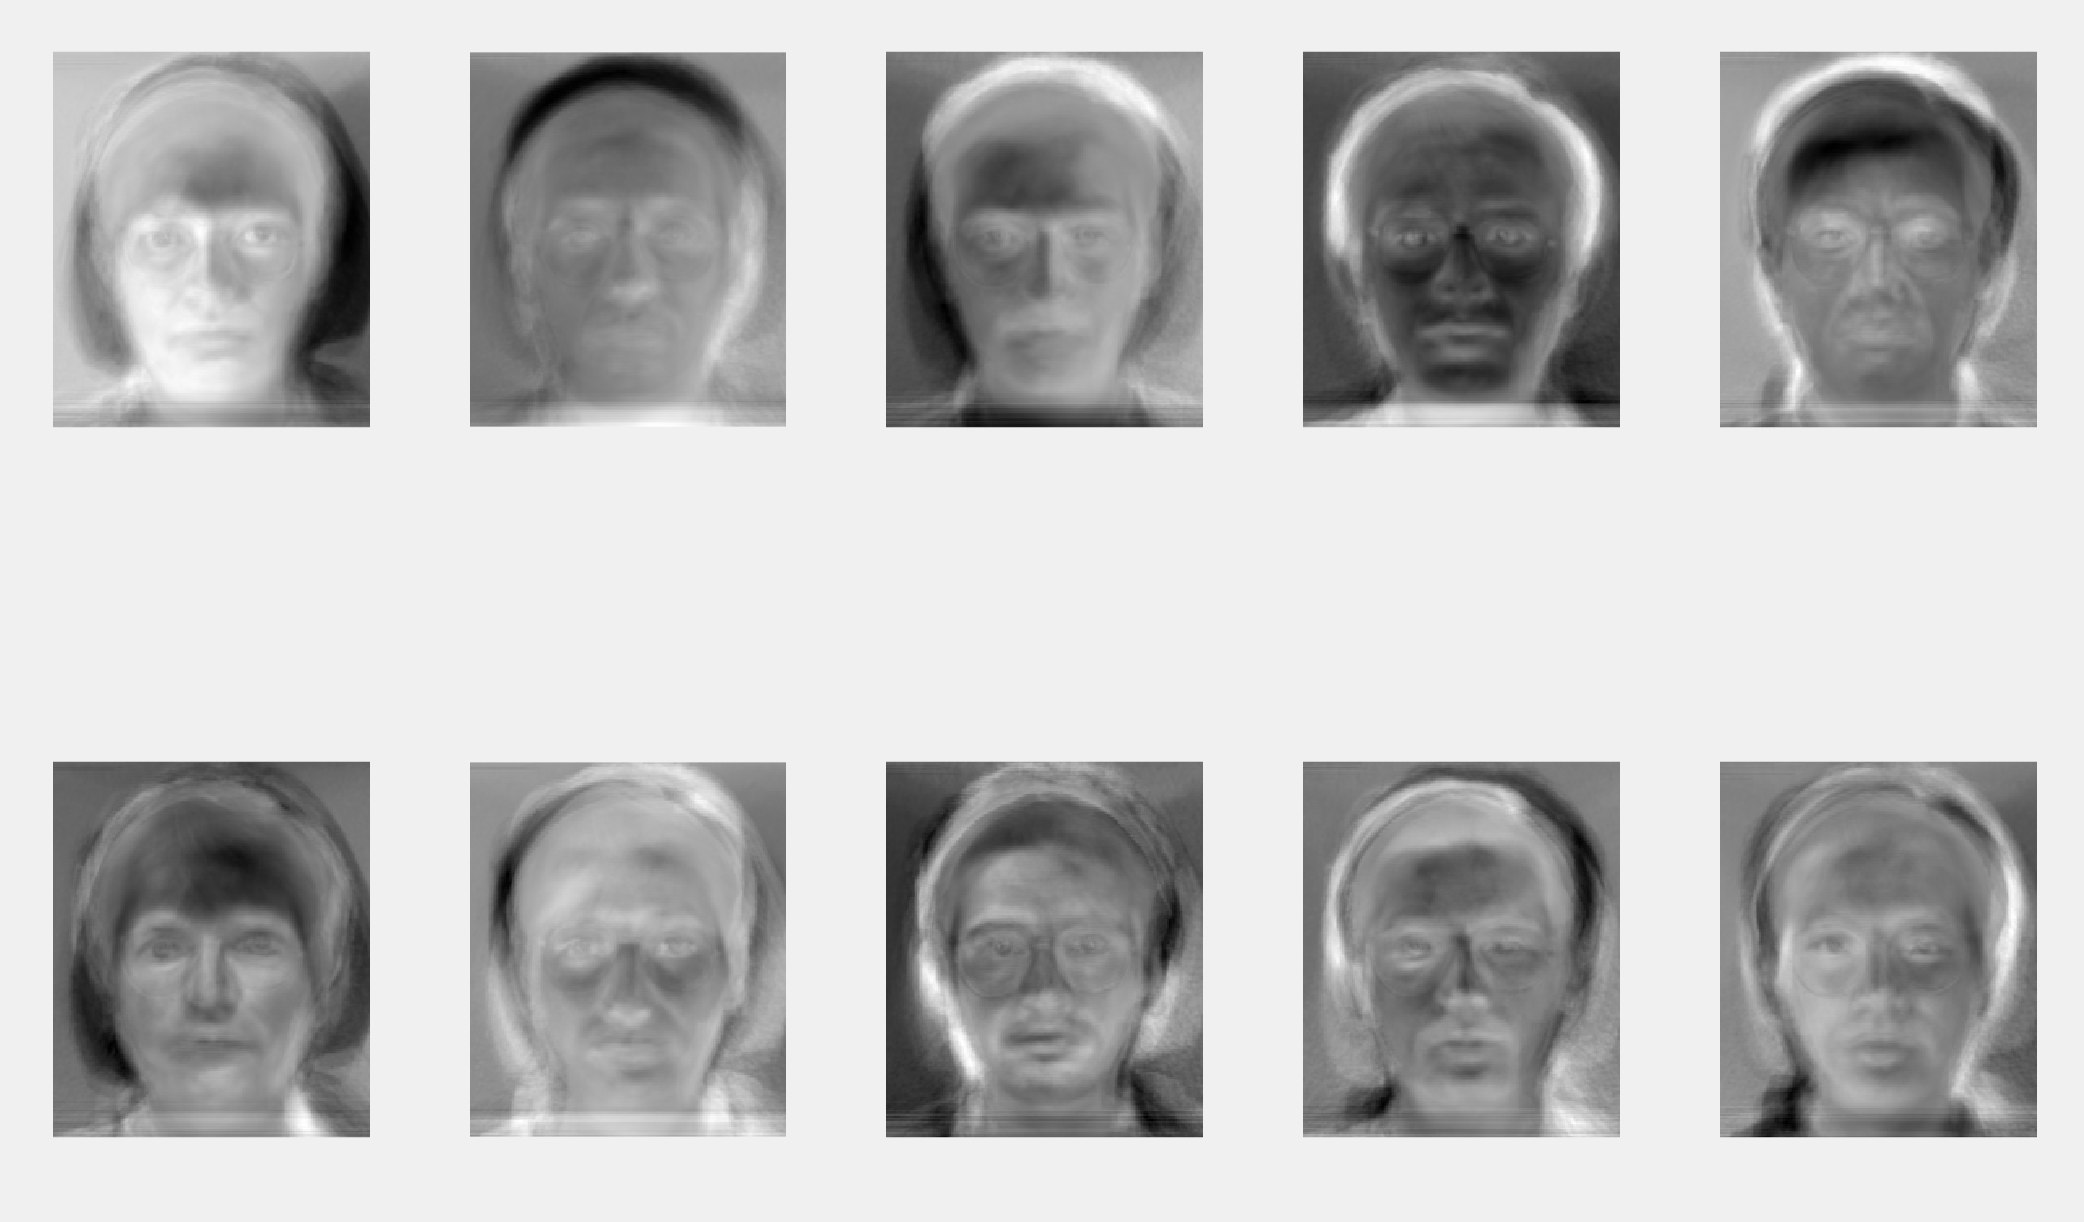
\includegraphics[scale = 0.25]{10.png}
    \caption{Top 10 eigenfaces}
    \label{fig6}
\end{figure}

\subsubsection*{Find the most similar faces for test images}

For this task, I first project all the training images to the eigenface space. Then for each test image, I also project it to the same space and calculate the Euclidean distance of the test image and all the training image points. Consider the three nearest points as the most similar images from the test image. The codes are listed below:

\begin{lstlisting}
%step 3: read in test images
test_name = './testset/';
test_dir = dir(test_name);
ll = length(test_dir);

%get the PCA coefficients of training images
PCA_coe = zeros(count,top);
for i = 1:count
    PCA_coe(i,:) = (train_matrix(:,i)'*eigen_face)/(eigen_face'*eigen_face);
end


%get similar faces
for i = 1:ll
    name = test_dir(i).name;
    if name(1)=='t'
        testg = imread([test_name,name]);
        figure;
        subplot(2,2,1);
        imshow(testg,[]);
        title('original imgae');
        testg = double(reshape(testg,[a*b,1]));
        testg = testg-mean_face;
        coordinates = testg'*eigen_face/(eigen_face'*eigen_face);
        distance = repmat(coordinates,count,1);
        distance = distance - PCA_coe;
        distance = distance.^2;
        distance = sum(distance,2);
        pos1 = find(distance == min(distance));
        pos1 = pos1(1);
        distance(pos1) = 9e+20;
        pos2 = find(distance == min(distance));
        pos2 = pos2(1);
        distance(pos2) = 9e+20;
        pos3 = find(distance == min(distance));
        pos3 = pos3(1);
        subplot(2,2,2);
        imshow(reshape(train_matrix(:,pos1)+mean_face,[a,b]),[]);
        title('The 1st similar image')
        subplot(2,2,3);
        imshow(reshape(train_matrix(:,pos2)+mean_face,[a,b]),[]);
        title('The 2nd similar image')
        subplot(2,2,4);
        imshow(reshape(train_matrix(:,pos3)+mean_face,[a,b]),[]);
        title('The 3rd similar image')
        
    end
end
\end{lstlisting}

Figure 7 to Figure 16 show the result of top 5 PC Analysis and Figure 17 to Figure 26 top 10 PC Analysis.

\begin{figure}[htbp]
\centering
\begin{minipage}[t]{0.48\textwidth}
\centering
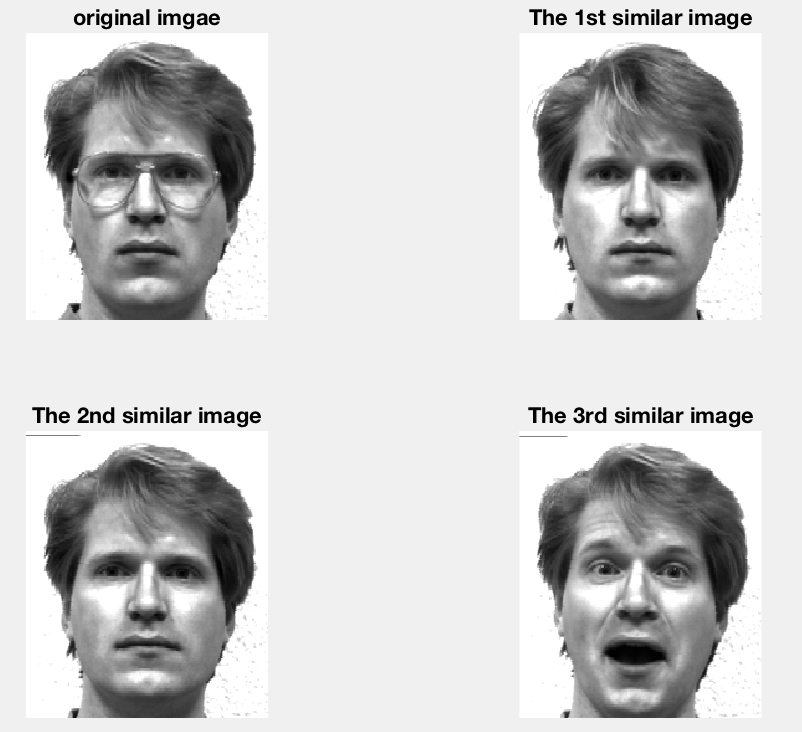
\includegraphics[scale = 0.3]{5_1.png}
\caption{Top 5 PCA on test 1}
\end{minipage}
\begin{minipage}[t]{0.48\textwidth}
\centering
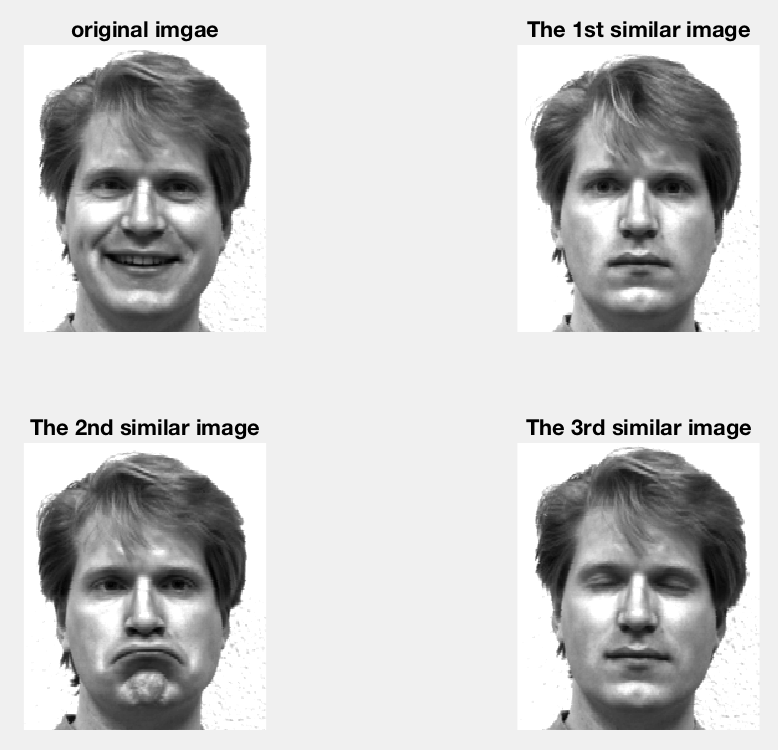
\includegraphics[scale = 0.3]{5_2.png}
\caption{Top 5 PCA on test 2}
\end{minipage}
\end{figure}

\begin{figure}[htbp]
\centering
\begin{minipage}[t]{0.48\textwidth}
\centering
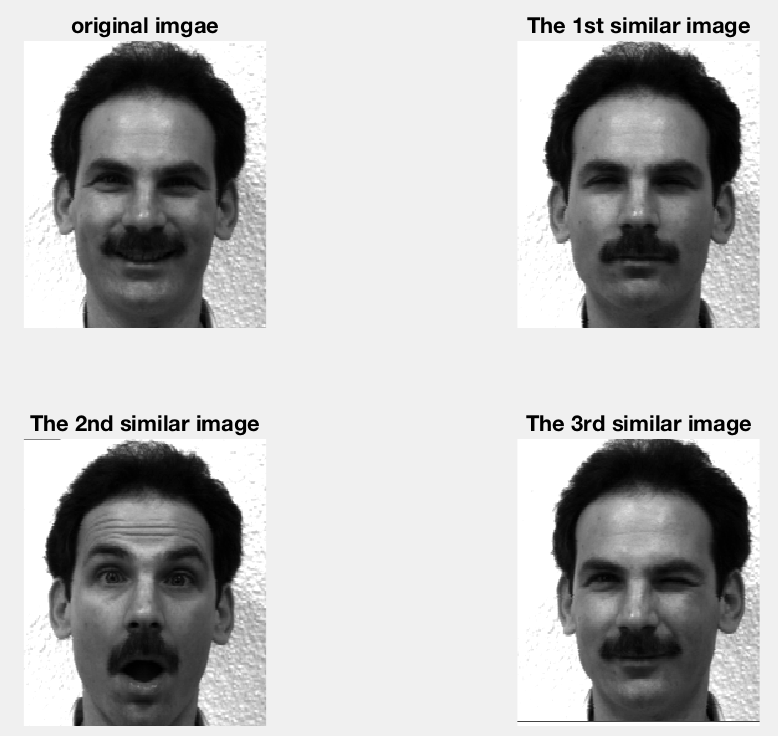
\includegraphics[scale = 0.3]{5_3.png}
\caption{Top 5 PCA on test 3}
\end{minipage}
\begin{minipage}[t]{0.48\textwidth}
\centering
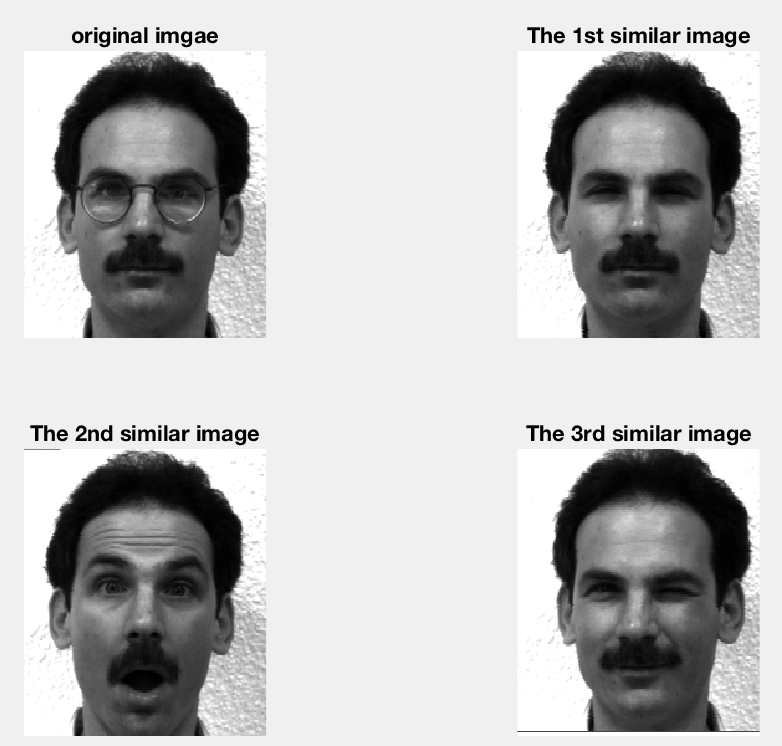
\includegraphics[scale = 0.3]{5_4.png}
\caption{Top 5 PCA on test 4}
\end{minipage}
\end{figure}

\begin{figure}[htbp]
\centering
\begin{minipage}[t]{0.48\textwidth}
\centering
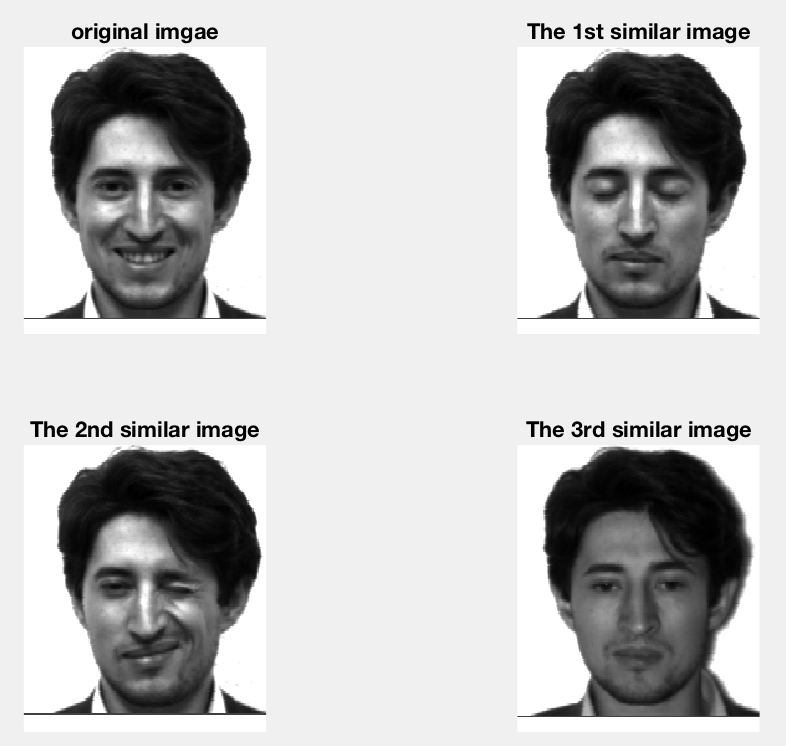
\includegraphics[scale = 0.3]{5_5.png}
\caption{Top 5 PCA on test 5}
\end{minipage}
\begin{minipage}[t]{0.48\textwidth}
\centering
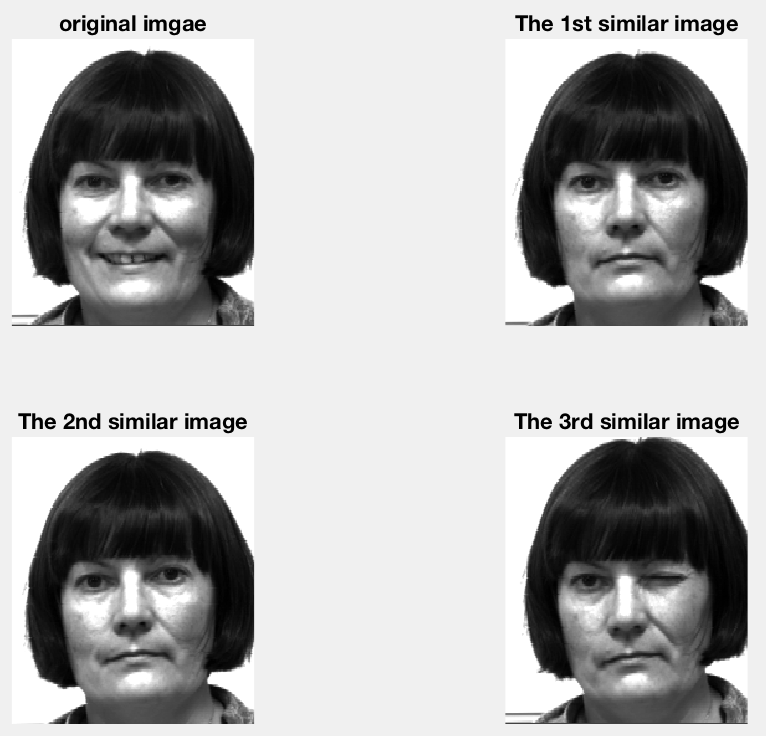
\includegraphics[scale = 0.3]{5_6.png}
\caption{Top 5 PCA on test 6}
\end{minipage}
\end{figure}

\begin{figure}[htbp]
\centering
\begin{minipage}[t]{0.48\textwidth}
\centering
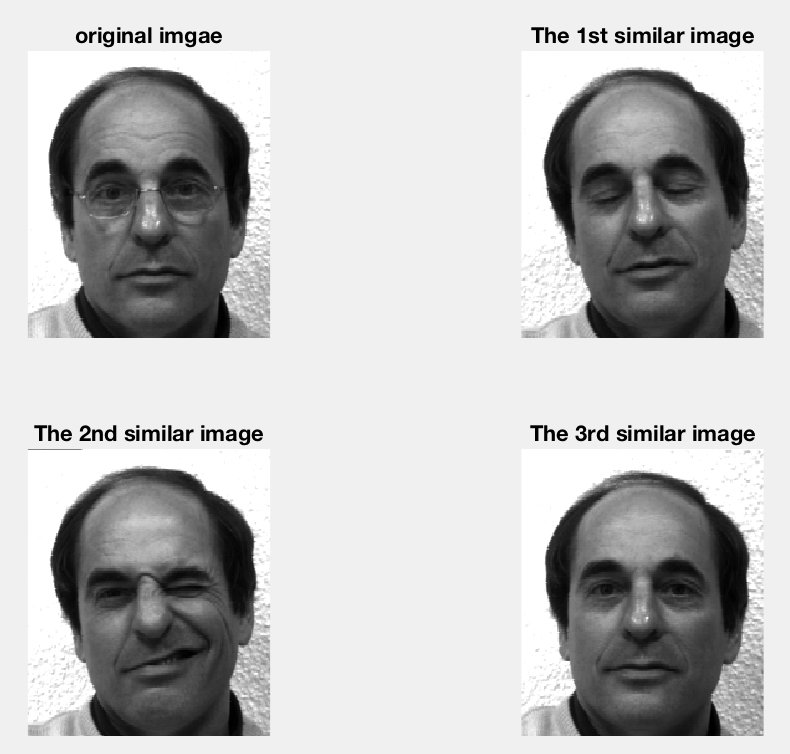
\includegraphics[scale = 0.3]{5_7.png}
\caption{Top 5 PCA on test 7}
\end{minipage}
\begin{minipage}[t]{0.48\textwidth}
\centering
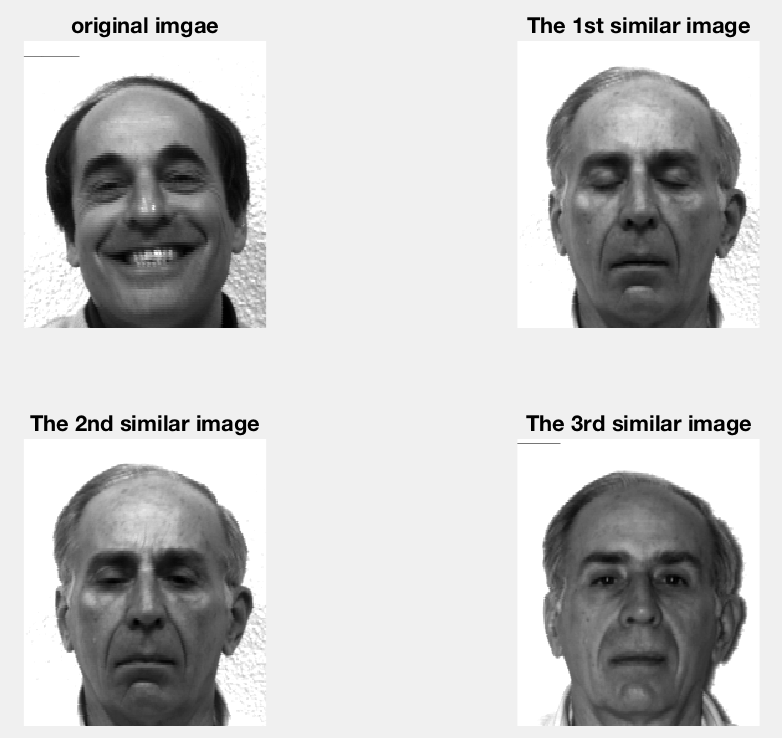
\includegraphics[scale = 0.3]{5_8.png}
\caption{Top 5 PCA on test 8}
\end{minipage}
\end{figure}

\begin{figure}[htbp]
\centering
\begin{minipage}[t]{0.48\textwidth}
\centering
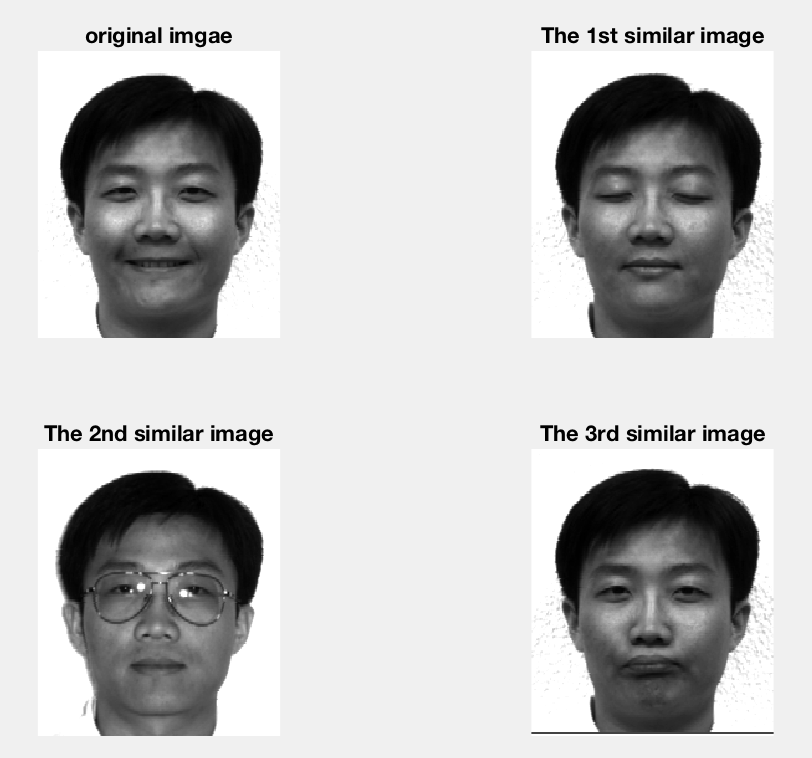
\includegraphics[scale = 0.3]{5_9.png}
\caption{Top 5 PCA on test 9}
\end{minipage}
\begin{minipage}[t]{0.48\textwidth}
\centering
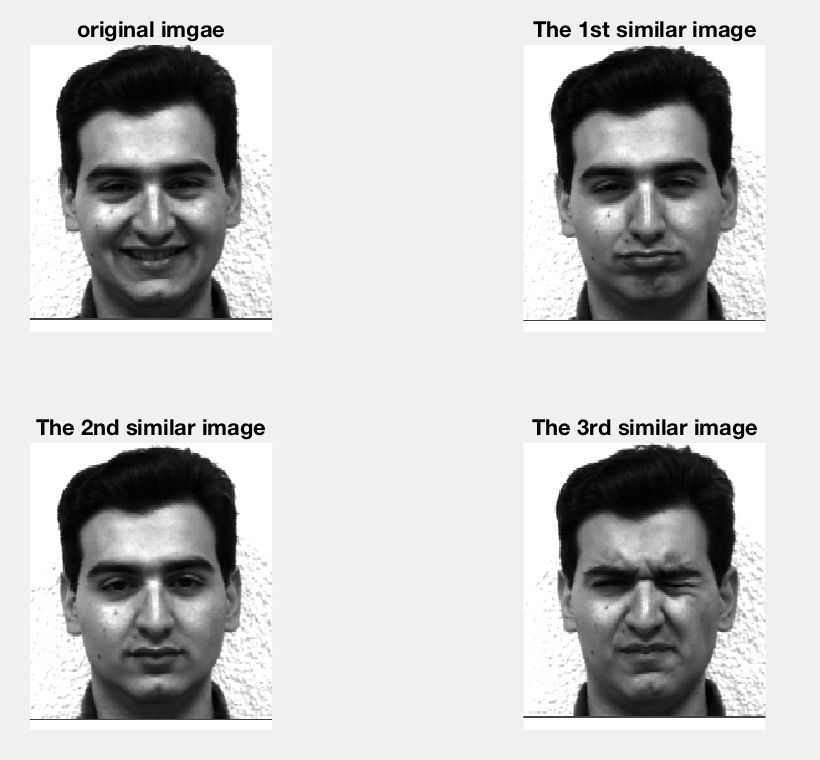
\includegraphics[scale = 0.3]{5_10.png}
\caption{Top 5 PCA on test 10}
\end{minipage}
\end{figure}

\begin{figure}[htbp]
\centering
\begin{minipage}[t]{0.48\textwidth}
\centering
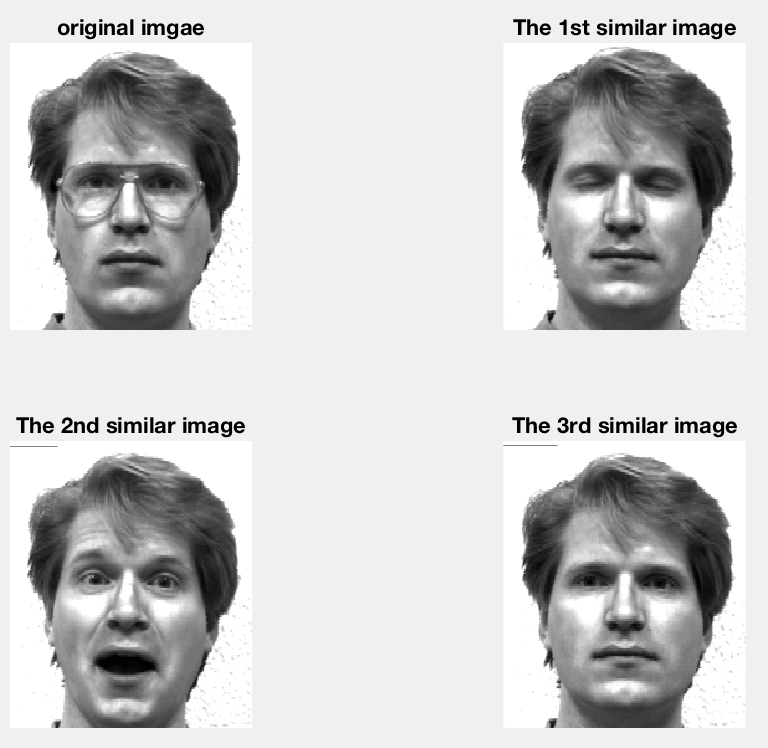
\includegraphics[scale = 0.3]{10_1.png}
\caption{Top 10 PCA on test 1}
\end{minipage}
\begin{minipage}[t]{0.48\textwidth}
\centering
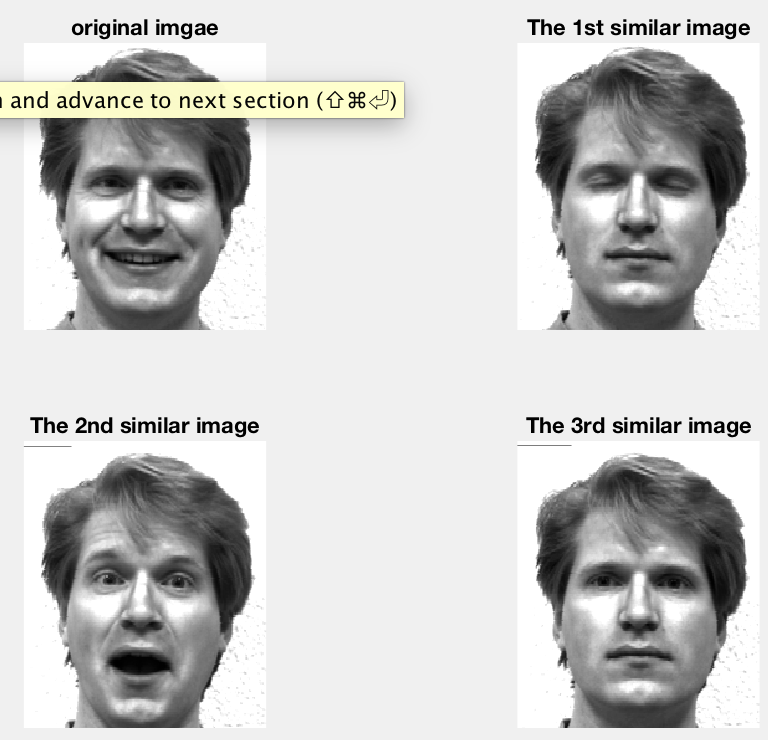
\includegraphics[scale = 0.3]{10_2.png}
\caption{Top 10 PCA on test 2}
\end{minipage}
\end{figure}

\begin{figure}[htbp]
\centering
\begin{minipage}[t]{0.48\textwidth}
\centering
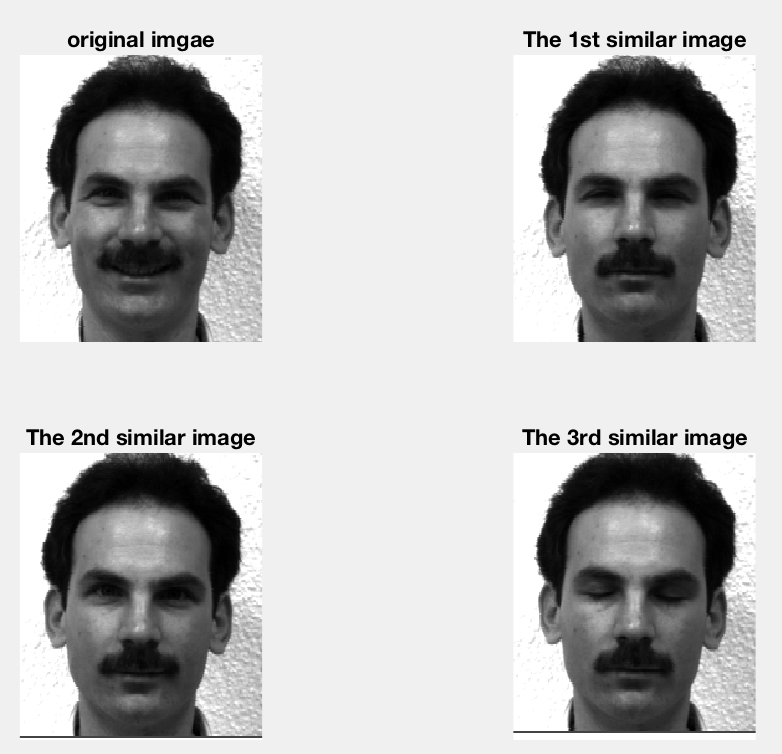
\includegraphics[scale = 0.3]{10_3.png}
\caption{Top 10 PCA on test 3}
\end{minipage}
\begin{minipage}[t]{0.48\textwidth}
\centering
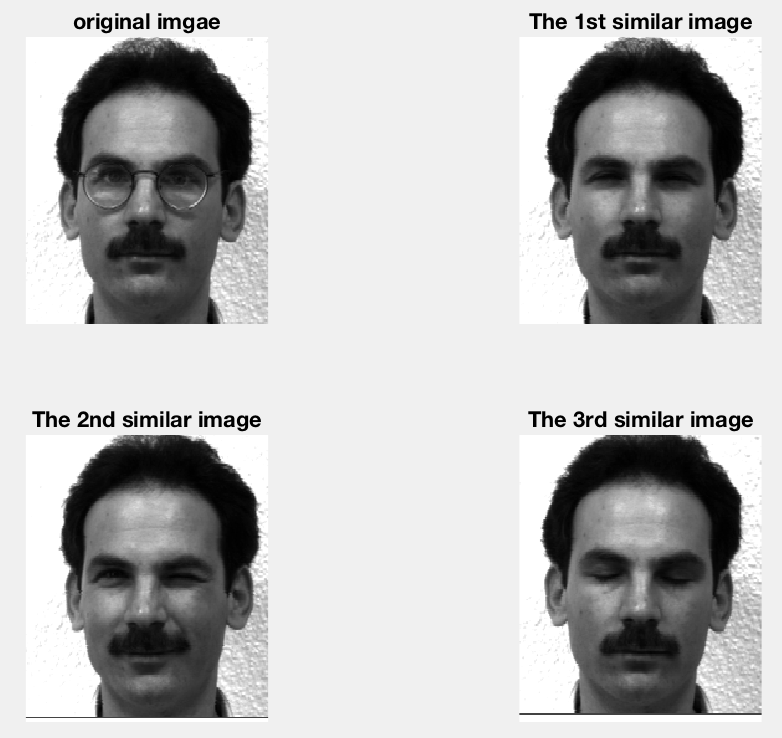
\includegraphics[scale = 0.3]{10_4.png}
\caption{Top 10 PCA on test 4}
\end{minipage}
\end{figure}

\begin{figure}[htbp]
\centering
\begin{minipage}[t]{0.48\textwidth}
\centering
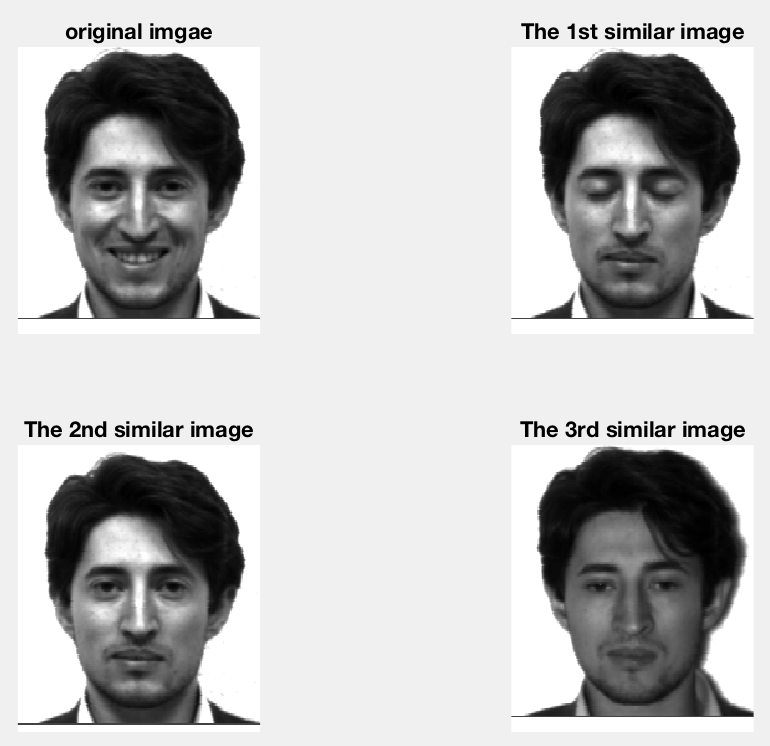
\includegraphics[scale = 0.3]{10_5.png}
\caption{Top 10 PCA on test 5}
\end{minipage}
\begin{minipage}[t]{0.48\textwidth}
\centering
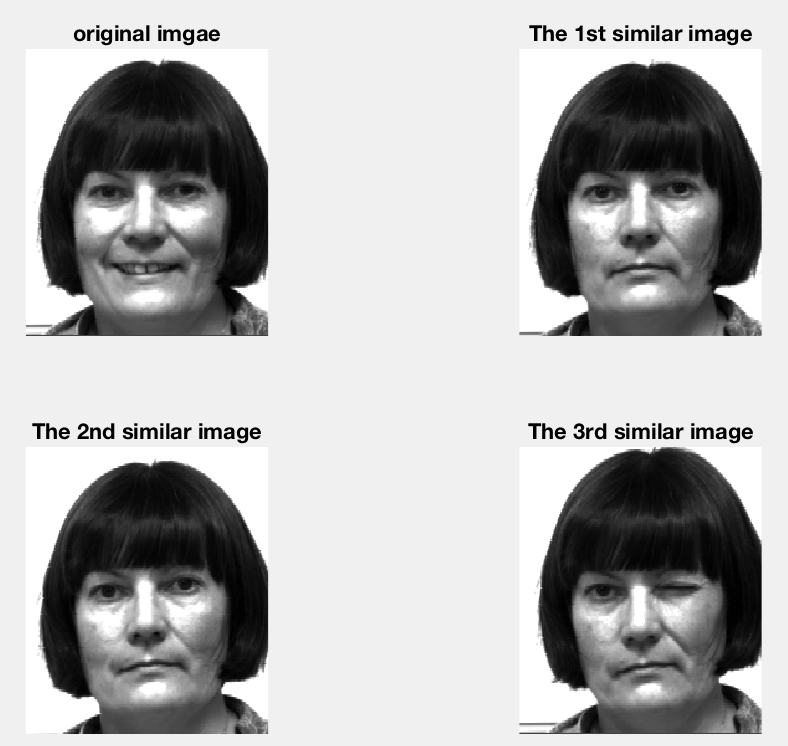
\includegraphics[scale = 0.3]{10_6.png}
\caption{Top 10 PCA on test 6}
\end{minipage}
\end{figure}

\begin{figure}[htbp]
\centering
\begin{minipage}[t]{0.48\textwidth}
\centering
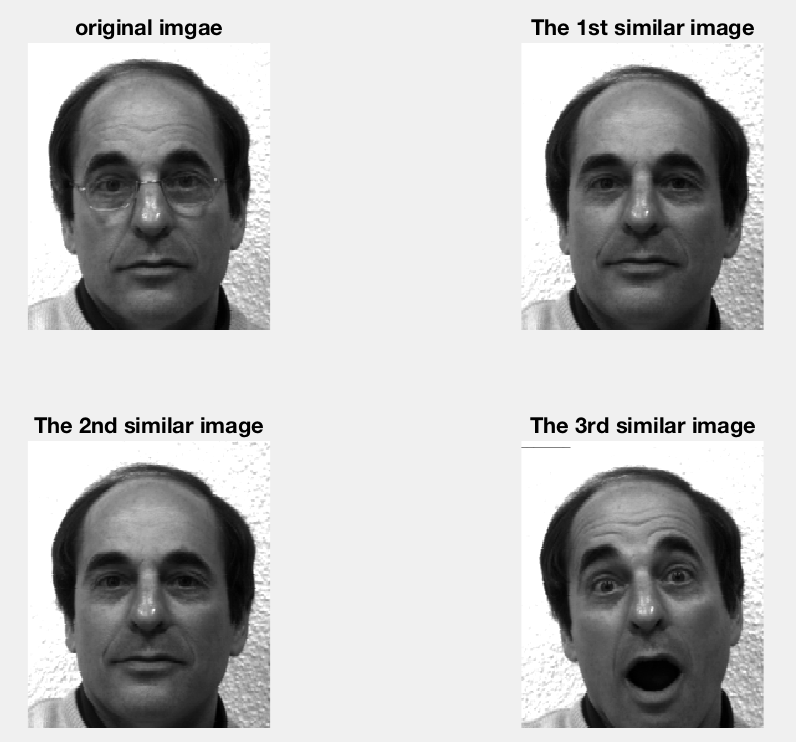
\includegraphics[scale = 0.3]{10_7.png}
\caption{Top 10 PCA on test 7}
\end{minipage}
\begin{minipage}[t]{0.48\textwidth}
\centering
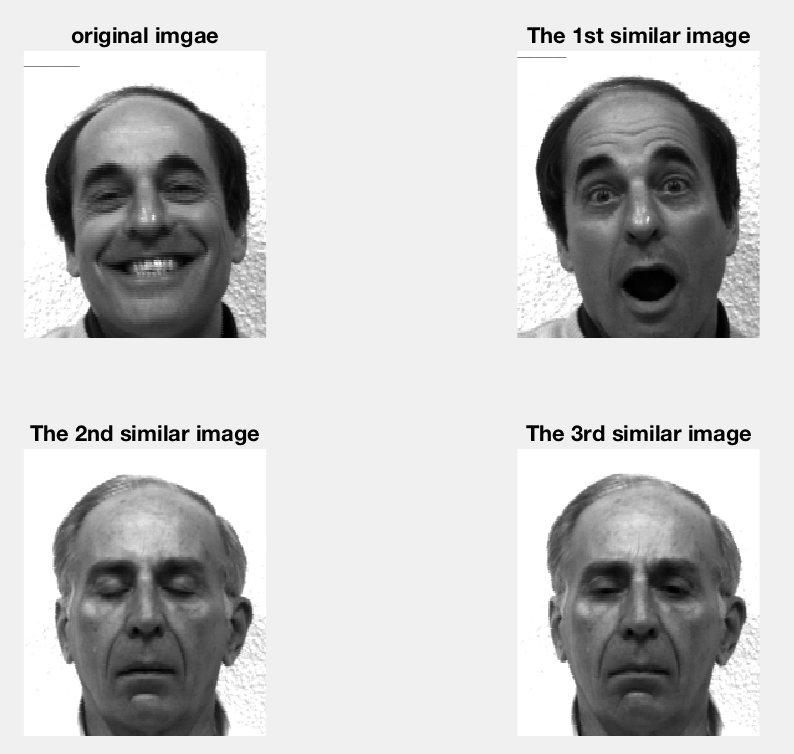
\includegraphics[scale = 0.3]{10_8.png}
\caption{Top 10 PCA on test 8}
\end{minipage}
\end{figure}

\begin{figure}[htbp]
\centering
\begin{minipage}[t]{0.48\textwidth}
\centering
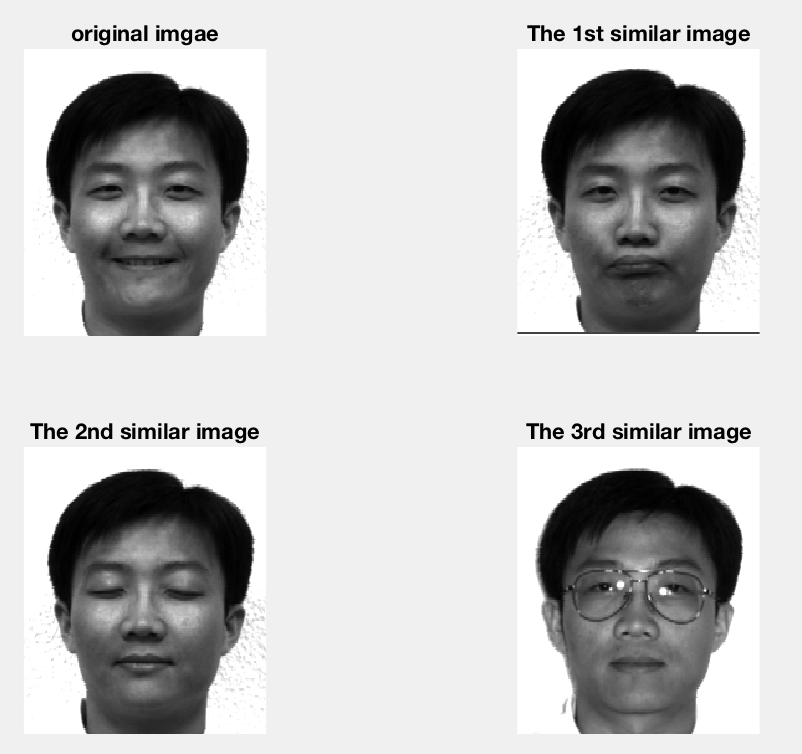
\includegraphics[scale = 0.3]{10_9.png}
\caption{Top 10 PCA on test 9}
\end{minipage}
\begin{minipage}[t]{0.48\textwidth}
\centering
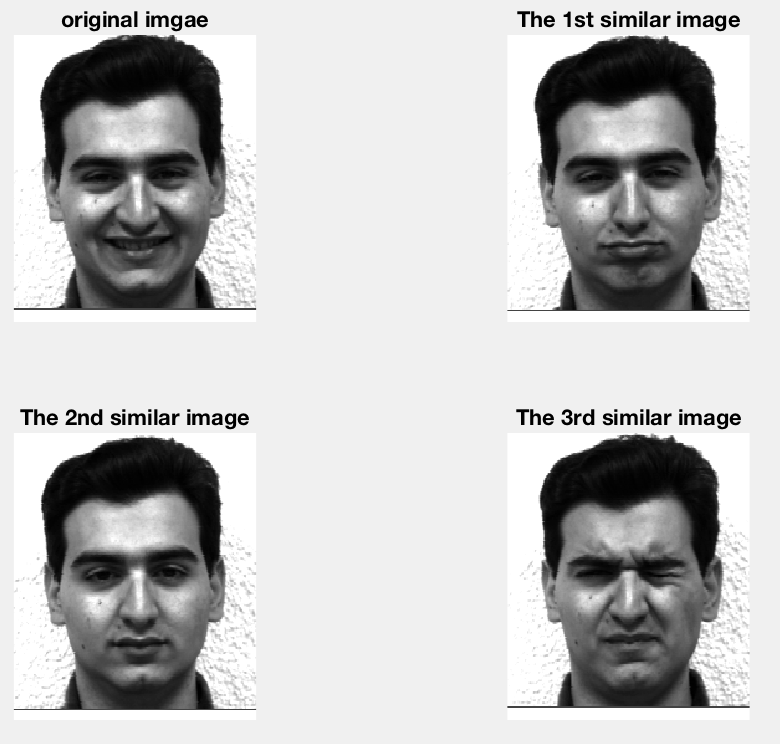
\includegraphics[scale = 0.3]{10_10.png}
\caption{Top 10 PCA on test 10}
\end{minipage}
\end{figure}

For the top 5 analysis, the overall recognition rate is \textbf{90\%}. All the images have the correct corresponding images except test image 8 which has totally wrong corresponding images. For the top 10 analysis, the overall recognition rate is \textbf{93.3\%}
The two mismatch pairs happened also on test image 8. Having a look at that specific result, we can see that the reason is that the two person is kind of similar in hairstyle and age. Even I saw them the first time, I thought they were the same person.

So personally speaking, I think the codes and results reflect the real ability of PCA in face recognition.

By the way, the most important thing in this task is to re-align the images. When I align the data by myself, the recognition rate stays at about 70\% to 80\%. When I align them with a Matlab script which means each image has the same standard format. In this situation, the recognition rate goes up to more than 90\%.

\section*{Task 2: DLT for 2-view homography estimation}

\subsubsection*{Find 6 pairs of corresponding points}
Using Matlab inbuilt function $ginput()$, we can get 6 pairs of corresponding points. Then I restore the data in order to make it convenient to debug. the locations of points 1 to points 6 are from upper left to the lower right.

The codes and results are listed below.

Codes:
\begin{lstlisting}
close all;
clear all;
clc;

im_left = imread('Left.jpg');
im_right = imread('Right.jpg');
figure;
subplot(1,2,1);
imshow(im_left);
title('Left Image');
subplot(1,2,2);
imshow(im_right);
title('Right Image');
hold on;
[x,y] = ginput(12);
\end{lstlisting}

Results:
\begin{figure}[htbp]
    \centering
    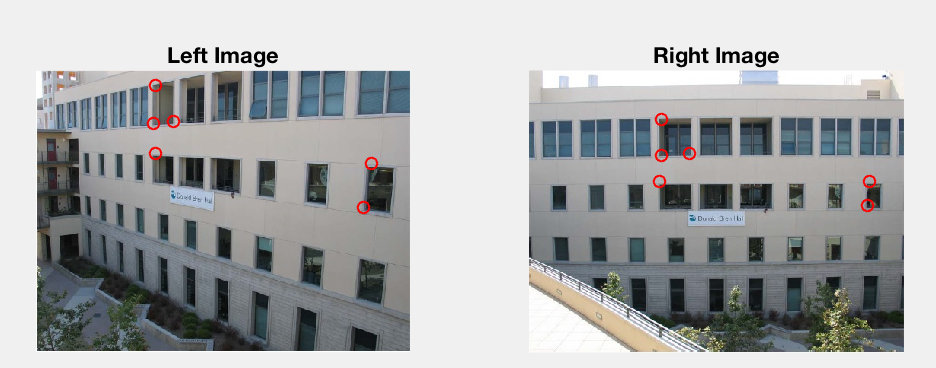
\includegraphics[scale = 0.6]{t2_1.png}
    \caption{Corresponding points of given images}
    \label{fig27}
\end{figure}

\subsubsection*{Step 2: Implement DLT.m}

The most important of DLT is to solve $H$ from the lecture we learned. 

First we know:

$$\begin{bmatrix}
x' \\ y' \\ 1 \end{bmatrix} = \left[ \begin{array}{ccc} h_{00} & h_{01} & h_{02} \\ h_{10} & h_{11} & h_{12} \\ h_{20} & h_{21} & h_{22} \end{array} \right] \times \left[ \begin{array}{c} x \\ y \\ 1 \end{array} \right]$$


After expose this equation, we can get following equations: 

\begin{equation*}
  \begin{aligned}
 		x'_{i}\times(h_{20}\times x_{i} + h_{21}\times y_{i} + h_{22}) = h_{00}\times x_{i} + h_{01}\times y_{i} + h_{02}\\
 		y'_{i}\times(h_{20}\times x_{i} + h_{21}\times y_{i} + h_{22}) = h_{10}\times x_{i} + h_{11}\times y_{i} + h_{12}\\
  \end{aligned}
  \label{eq1}
\end{equation*}

Then, the problem become to get the eigenvector that belongs to the smallest eigenvalue of matrix A.

$$A = \begin{bmatrix} x_{1} & y_{1} & 1 & 0 & 0 & 0 & -x'_{1}x_{1} & -x'_{1} y_{1} & -x'_{1} \\ 0 & 0 & 0 & x_{1} & y_{1} & 1 &  -y'_{1} x_{1} & -y'_{1} y_{1} & -y'_{1} \\ ...  \\ x_{i} & y_{i} & 1 & 0 & 0 & 0 & -x'_{i}x_{i} & -x'_{i} y_{i} & -x'_{i} \\ 0 & 0 & 0 & x_{i} & y_{i} & 1 &  -y'_{i} x_{i} & -y'_{i} y_{i} & -y'_{i} \end{bmatrix} $$

Based on these knowledge from the lecture, I implement the DLT function. 

The codes are listed below:

\begin{lstlisting}

function H=DLT(u2Trans, v2Trans, uBase, vBase)
% Computes the homography H applying the Direct Linear Transformation
% The transformation is such that
% p = H p' , i.e.,:
% (uBase, vBase, 1)'=H*(u2Trans , v2Trans, 1)' %
% INPUTS:
% u2Trans, v2Trans - vectors with coordinates u and v of the transformed image point (p')
% uBase, vBase - vectors with coordinates u and v of the original base image point p
%
% OUTPUT
% H - a 3x3 Homography matrix %
% Zhipeng Bao 27th Apr, 2018
l = length(uBase);
% assume the length of u2Tran, v2Tran, uBase, vBase are the same, or we need
% to write some codes for anomaly detection.
A = zeros(2*l,9);
%Form the matrix A;
for i = 1:l
    x = u2Trans(i);
    y = v2Trans(i);
    xp = uBase(i);
    yp = vBase(i);
    A(2*i-1,:) =  [x,y,1,0,0,0,-xp*x,-xp*y,-xp];
    A(2*i,:) = [0,0,0,x,y,1,-yp*x,-yp*y,-yp];
end
%svd decompose
[S,D,V] = svd(A);
[w,h] = size(V);
%get the last column of V matrix which is H
H = V(:,end);
%reshape H to 3X3
H = reshape(H,[3 3])';
%Normalize H
H = H/H(3,3);

\end{lstlisting}

\subsubsection*{Step 3: Test results}

By running the DLT function, we can get the result of H. It displays as the following:

$$H = \begin{bmatrix} 0.2572 & 0.0712 & 75.1127 \\ -0.1244 & 0.9802 & -21.5698 \\ -0.0013 & 0.0004 & 1.0000 \end{bmatrix} $$

To verify the H matrix, I find the projective image from the right image based on H and show the result below.

\begin{figure}[htbp]
    \centering
    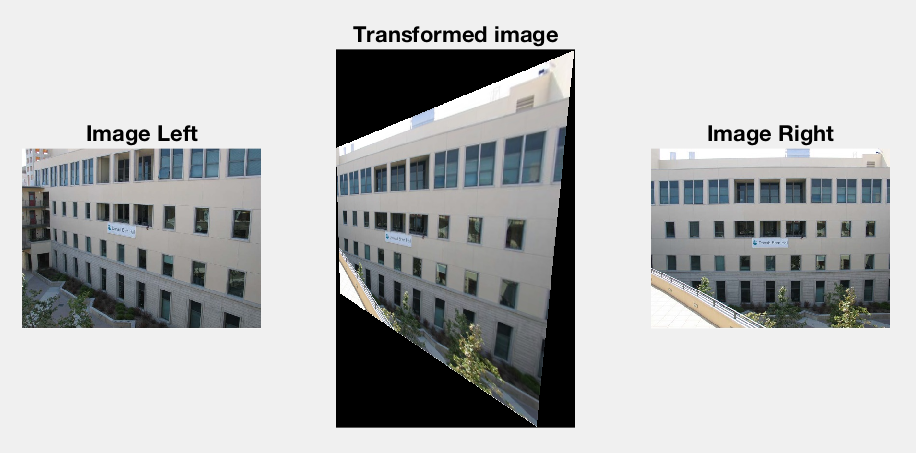
\includegraphics[scale = 0.6]{t2_2.png}
    \caption{Transformed result}
    \label{fig28}
\end{figure}

The first two images shared almost the same perspective which proves the correctness of the codes.

\subsubsection*{how many points are minimally required in order to apply DLT to estimate a Homography}

At list 4 pairs of points are needed to apply DLT algorithm. The reason is that the matrix H has 8 degrees of freedom and each pair of points can provide two linear independent equations. Thus, to solve all the 8 degrees, at least 4 pairs of points are needed.

I also test the 4 points in my Matlab experiments, I firstly select point 1,3,4,6 to get the result. It shows below:

$$H = \begin{bmatrix} 0.2765 & -0.0097 & 76.7986 \\ -0.1067 & 0.8509 & -20.9564 \\ -0.0012 & 0.0002 & 1.0000 \end{bmatrix} $$

\begin{figure}[htbp]
    \centering
    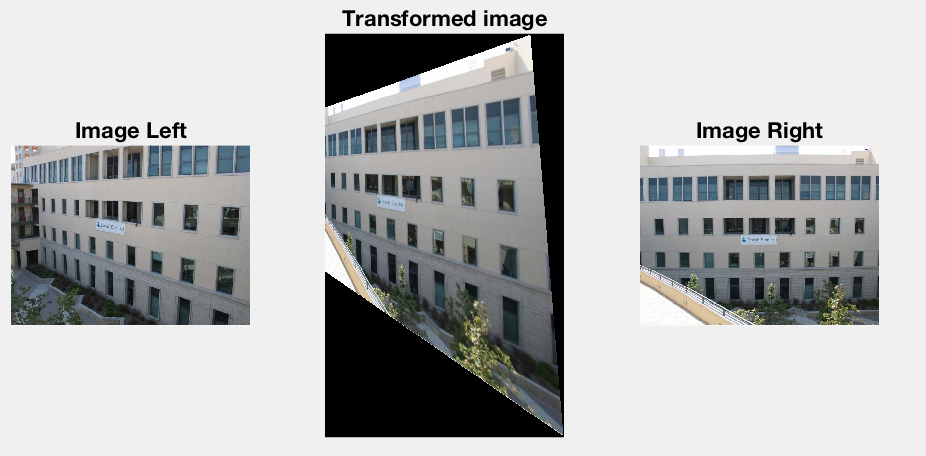
\includegraphics[scale = 0.6]{t2_3.png}
    \caption{Result based on pairs 1,3,4,5}
    \label{fig29}
\end{figure}

The result is quite similar to the 6-pair one. So it is proved 4 pairs of points is enough to estimate matrix $H$.

However, to keep the DLT method robust, we need to give more points. For example, if I use the pairs [1,2,3,5], in which points 1,2,3 are concentrating on the same area, to estimate matrix $H$, the result is not that good. Here are the results.

$$H = \begin{bmatrix} 0.3939 & 0.2485 & 50.3797 \\ -0.1054 & 1.0403 & -32.1165 \\ -0.0015 & 0.0019 & 1.0000 \end{bmatrix} $$

\begin{figure}[htbp]
    \centering
    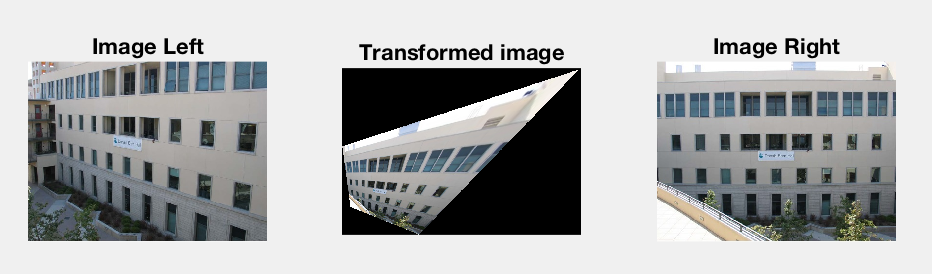
\includegraphics[scale = 0.6]{t2_4.png}
    \caption{Result based on pairs 1,2,3,5}
    \label{fig30}
\end{figure}

In conclusion, we need at least 4 pair of points to apply DLT method. But to get an effective DLT result, the locations of the pairs should be decentralized. With more pairs of points, the result will be more accurate.

\section*{Attached codes}
For this part, I attach the main codes of each task and some other supportive codes here.

\subsubsection*{Task1.m}
\begin{lstlisting}
clear all;
close all;
clc;

%step1: have a look at the training images
dir_name = './trainingset/';
dir_lst = dir(dir_name);
l = length(dir_lst);

top = 10;

%step2: train eigenfaces
train_matrix = [];
count = 0;
%get the train matrix
for i = 1:l
   name = dir_lst(i).name;
   if name(1)=='s'
       img = imread([dir_name,name]);
       [a,b] = size(img);
       img = reshape(img,[a*b 1]);
       img = double(img);
       train_matrix = [train_matrix,img];
       count = count+1;
   end
end

%remove DC Component
mean_face = mean(train_matrix,2);
train_matrix = train_matrix - repmat(mean_face,1,count);

%tricky: A'A and AA' have the same eigen value
%and their eigen vector can be transformed.
A = train_matrix'*train_matrix;
eigen_face = eigenfaces(A,top);

%actual eigen vectors(faces).
eigen_face = train_matrix*eigen_face;

%show eigen faces
figure;
for i = 1: top
   subplot(2,ceil(top/2),i);
   imshow(reshape(eigen_face(:,i),[a,b]),[]);
end

%step 3: read in test images
test_name = './testset/';
test_dir = dir(test_name);
ll = length(test_dir);

%get the PCA coefficients of training images
PCA_coe = zeros(count,top);
for i = 1:count
    PCA_coe(i,:) = (train_matrix(:,i)'*eigen_face)/(eigen_face'*eigen_face);
end


%get similar faces
for i = 1:ll
    name = test_dir(i).name;
    if name(1)=='t'
        test_img = imread([test_name,name]);
        figure;
        subplot(2,2,1);
        imshow(test_img,[]);
        title('original imgae');
        test_img = double(reshape(test_img,[a*b,1]));
        test_img = test_img-mean_face;
        coordinates = test_img'*eigen_face/(eigen_face'*eigen_face);
        distance = repmat(coordinates,count,1);
        distance = distance - PCA_coe;
        distance = distance.^2;
        distance = sum(distance,2);
        pos1 = find(distance == min(distance));
        pos1 = pos1(1);
        distance(pos1) = 9e+20;
        pos2 = find(distance == min(distance));
        pos2 = pos2(1);
        distance(pos2) = 9e+20;
        pos3 = find(distance == min(distance));
        pos3 = pos3(1);
        subplot(2,2,2);
        imshow(reshape(train_matrix(:,pos1)+mean_face,[a,b]),[]);
        title('The 1st similar image')
        subplot(2,2,3);
        imshow(reshape(train_matrix(:,pos2)+mean_face,[a,b]),[]);
        title('The 2nd similar image')
        subplot(2,2,4);
        imshow(reshape(train_matrix(:,pos3)+mean_face,[a,b]),[]);
        title('The 3rd similar image')
        
    end
end
\end{lstlisting}

\subsubsection*{Task2.m}
\begin{lstlisting}
close all;
clear all;
clc;

im_left = imread('Left.jpg');
im_right = imread('Right.jpg');
%{
figure;
subplot(1,2,1);
imshow(im_left);
title('Left Image');
subplot(1,2,2);
imshow(im_right);
title('Right Image');
hold on;
[x,y] = ginput(12);
%}
%load data
load t2.mat;
a = [1,3,5,7,9,11];
b = [2,4,6,8,10,12];
x1 = x(a);
x2 = x(b);
y1 = y(a);
y2 = y(b);
H = DLT(x2,y2,x1,y1);
disp('H = ');
disp(H);


figure;
tform = projective2d(H');
imageTrans = imwarp(im_right,tform);
subplot(1,3,1);
imshow(im_left);
title('Image Left');
subplot(1,3,2);
imshow(imageTrans,[]);
title('Transformed image');
subplot(1,3,3);
imshow(im_right);
title('Image Right');
\end{lstlisting}

\subsubsection*{DLT.m}
\begin{lstlisting}
function H=DLT(u2Trans, v2Trans, uBase, vBase)
% Computes the homography H applying the Direct Linear Transformation
% The transformation is such that
% p = H p' , i.e.,:
% (uBase, vBase, 1)'=H*(u2Trans , v2Trans, 1)' %
% INPUTS:
% u2Trans, v2Trans - vectors with coordinates u and v of the transformed image point (p')
% uBase, vBase - vectors with coordinates u and v of the original base image point p
%
% OUTPUT
% H - a 3x3 Homography matrix %
% Zhipeng Bao 27th Apr, 2018
l = length(uBase);
% assume the length of u2Tran, v2Tran, uBase, vBase are the same, or we need
% to write some codes for anomaly detection.
A = zeros(2*l,9);
%Form the matrix A;
for i = 1:l
    x = u2Trans(i);
    y = v2Trans(i);
    xp = uBase(i);
    yp = vBase(i);
    A(2*i-1,:) =  [x,y,1,0,0,0,-xp*x,-xp*y,-xp];
    A(2*i,:) = [0,0,0,x,y,1,-yp*x,-yp*y,-yp];
end
%svd decompose
[S,D,V] = svd(A);
[w,h] = size(V);
%get the last column of V matrix which is H
H = V(:,end);
%reshape H to 3X3
H = reshape(H,[3 3])';
%Normalize H
H = H/H(3,3);

\end{lstlisting}

\end{document}


